\section{Experimental Setup}
\label{exp}

\subsection{Dataset}
%no hablar mucho de etiquetas puesto que es solo para evaluacion... es una tecncia no supervisada.
%Currently, the dataset with the most studied exoplanets is from the NASA based on the effectiveness of Kepler mission\footnote{Kepler measured the light variation of thousand of distant stars in search of periodic planetary transit within our galaxy neighborhood.}. Particularly,

Our work uses the \textit{Kepler Objects of Interest} (KOI) dataset\footnote{http://archive.stsci.edu/search\_fields.php?mission=kepler\_koi} provided by MAST (\textit{Mikulski Archive for Space Telescopes}) \citep{akeson2013nasa}. It is composed by 8054 records where every Kepler Object of Interest (KOI) is a region of interest in the sky that shows a periodic behavior based on thresholding events. These objects are categorized according to Nasa Exoplanet Science Institute\footnote{http://nexsci.caltech.edu/}, as \textit{Confirmed}, claimed exoplanets through extensive scientific analysis and follow ups; \textit{False Positive}, initially selected as candidate exoplanets but additional evidence show they are not; or \textit{Candidate}, those that are still under study (unlabeled data).
Multiple KOIs are obtained from each host star, and each object contains raw measurements with timestamps, including the instrumental error associated to each measure. The sampling rate is 0.0204 BJD on average (i.e., half an hour), but there is a 22.98\% of missing values per light curve on average. Each light curve has approximately 55000 effective measurements.

The archive also provides a set of metadata values, some of them (usually related to the star) are cross-matched from other catalogues. For comparing our self-generated features with model-based ones, we have selected only those that can be directly obtained from the light curves by following the Mandel-Agol model \citep{mandel2002analytic}.
%\emph{period}, \emph{First Transit Time}

%\subsubsection*{\textbf{Metadata}}
%From all the high-level features (metadata) that was available, we have selected the features that can be extracted only from the light curve, without cross-matching from other cataloges.
%\begin{itemize}
%\item \emph{Period}: the interval between consecutive planetary transits in days. Calculated as one of the best-fit parameter on a Mandel-Agol model \citep{mandel2002analytic}.
%\item \emph{First Transit Time}: the time when the exoplanet pass in front of the host star in BJD. Calculated as one of the best-fit parameter on a Mandel-Agol model \citep{mandel2002analytic}.
%\item \emph{Inclination}: the angle between the plane of the sky (perpendicular to the line of sight) and the orbital plane of the object (90 degrees is a orbit in the line of sight). Calculated as one of the best-fit parameter on a Mandel-Agol model \citep{mandel2002analytic}.
%\item \emph{Planet Radius} (over Stellar Radius): the inferred radius of the Object of Interest. Based on a best-fit parameter on a Mandel-Agol model \citep{mandel2002analytic}. Calculated as one of the best-fit parameter on a Mandel-Agol model \citep{mandel2002analytic}.
%\item \emph{Semi-major Axis} (over Stellar Radius): orbital radius based on the axis of an elliptic orbit. Calculated as one of the best-fit parameter on a Mandel-Agol model \citep{mandel2002analytic}.
%\item \emph{Limb Darkening Coefficients}: models the light variation (darkening) on the edges of the star, two coefficient (linear and quadratic). To be sure, Kepler used cross-matching.

%\item \emph{Impact Parameter}: distance between the object and the sight axis to the star. Calculated based on the orbit radius and the inclination.
%\item \emph{Transit Duration}: time between first contact and last contact in days (eclipse duration). Calculated based on the transit period, planet radius and orbit radius.
%\item \emph{Fitted stellar density}: calculated based on a small planet approximation with the planet radius, transit period and duration.
%\item \emph{Planet Teq}: the expected temperature of equilibrium on the surface of the candidate planet in Kelvin. Calculated through the stellar temperature and the planet's radiation.
%\end{itemize}


%\subsection{Dataset Pre-processing}
We use Kepler's detrend pipeline \citep{fanelli2011kepler} to obtain a standard light curve for our experiments, i.e. that express the changes respect to a local window behavior. It consist on applying
%\begin{enumerate}
%    \item Apply 
a polynomial fit, Sav-Gol filter \citep{savitzky1964smoothing}, of 2 degrees with a window of 151, and then subtract it to the light curve. Then it
   % \item Apply  and 
subtracts a moving median filter, with a window of 25.
Finally, we removes
%    \item Remove 
positive outliers that are high than $5\sigma$ and removes negative outliers lower than $40 \sigma$. 
%With $\sigma$ the standard deviation of the light curve.
%\end{enumerate}


\subsection{Data Representation}
\begin{figure}[!t]
    \centering
    \begin{tabular}{c}
        Example 1 \\
         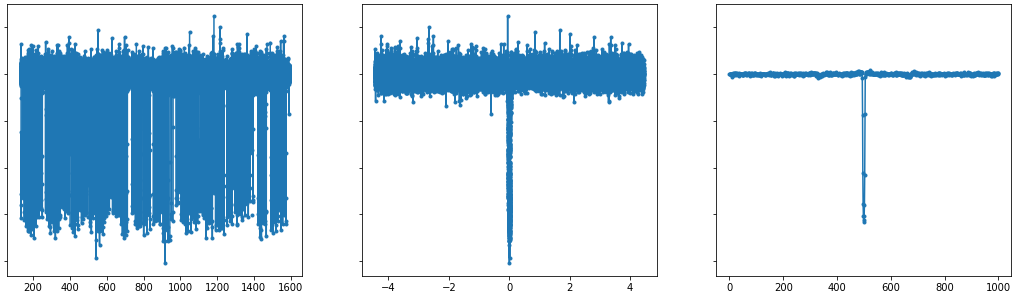
\includegraphics[width=0.95\textwidth, height=3cm]{imgs/conf_ex.png}  \\
        Example 2 \\ 
         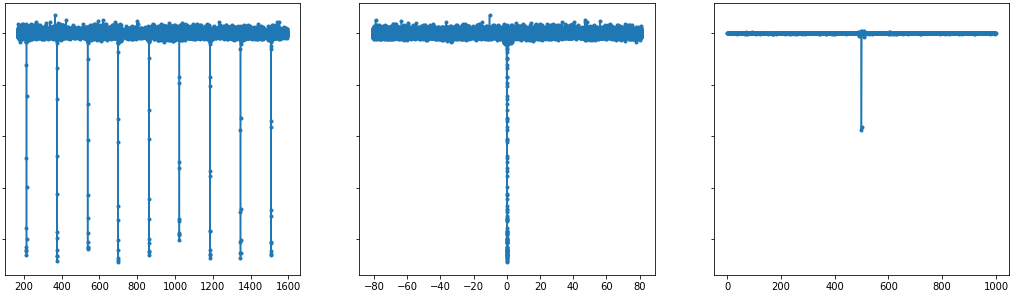
\includegraphics[width=0.95\textwidth, height=3cm]{imgs/narrow_ex.png} \\
         Example 3 \\ 
         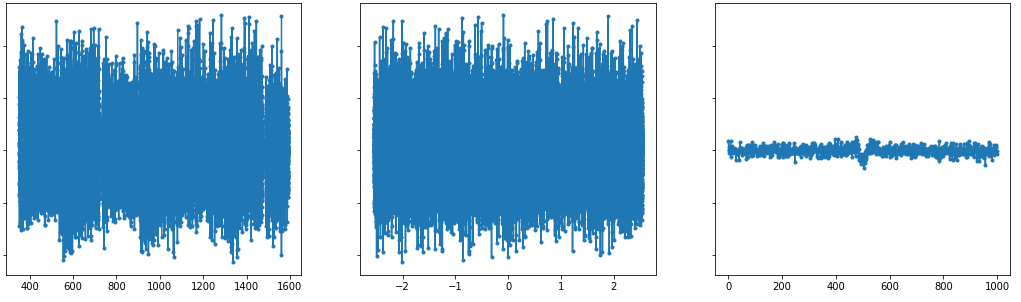
\includegraphics[width=0.95\textwidth, height=3cm]{imgs/noisy_ex.png} 
    \end{tabular}
    \caption{Examples on the different representation that can be obtained from a periodic light curve by knowing the period $P$. The images on every example is the raw light curve, the folded and folded-global (setting the bins to $T=1000$) on the columns respectively. The third column is the representation used on this work.}
    \label{fig:representation_ex}
\end{figure}

For the light curve measurement $x^{(i)}$, we use the \textbf{folded-global} representation proposed by \citep{shallue2018identifying}. First it produce a vector $f^{(i)}$ with the same number of points by folding the raw light curve on the period ($P$), with the event centered (fold step). Then, a windowed median is applied every $P/T$ times over the folded light curve $f^{(i)}$ (global step). This produces a vector $\mathbf{x}^{(i)}$ with $T$ points, so each light curve has the same length with the width interval depending on the period $P$.
%This representation was original used to classify \textit{Thresholding Crossing Event} (TCE)\footnote{This is detect Candidates from False Positive objects} with a good performance. The process is described here:
%\begin{enumerate}
%    \item \textit{Fold}: Produce a vector $f^{(i)}$ with the same number of points by folding the raw light curve on the period ($P$), with the event centered (need the \textit{first time transit} measure).
%    \item \textit{Global}: A window median is applied every $P/T$ times, on the folded light curve $f^{(i)}$. Producing a vector $\mathbf{x}^{(i)}$ with $T$ points, so each light curve has the same length with the width interval depending on the period $P$.
%\end{enumerate}
The parameter $T$ controls the trade-off between a detailed representation and having enough points on each window for the median to be meaningful.

Figure \ref{fig:representation_ex} shows examples of folded and folded-global representations of light curves.
The second example illustrates a general disadvantage of this method, where long-period KOIs may end up with very narrow transits that fall entirely within a small number of bins. On the other hand, the third example shows how the folded-global representation helps to get a more cleaned version of the light curve when the planets are small. 

As explained in Section~\ref{proposal}, the delta times ($\delta^{(i)}$) of the folded-global representation are considered as an additional input for the learning models. 
Also, please recall that the light curve measurements $\mathbf{x}^{(i)}$ are previously normalized through $\mathbf{x}'^{(i)} = \mathbf{x}^{(i)}/std(\mathbf{x}^{(i)})$ for VRAE$_t$,%, as pre-process let the light curves centered ($mean(\mathbf{x}^{(i)}) = 0 \ \forall i$). 
while the raw light curve measurements $\mathbf{x}^{(i)}$ are used for the proposed S-VRAE$_t$ model.


\subsection{Data Selection and Augmentation} %and Further Processes
%We set a mask over all the objects on Kepler mission (8054 records) to filter out light curves without a transit behavior, obtaining 4317 objects to train our models. 
%Concretely, we remove objects that either (i) are classified as ``secondary transit" or ``not transit", (ii) have a \textit{transit score} lower than $0.55$, or (iii) have a Mandel-Agol residual higher than $1$.
%The candidates objects that are not transit could be because the transit was from another object (non-planetary) in the background or because it was a binary system, i.e. two stars orbiting around their barycenter.

We set a mask over all the objects on Kepler mission (8054 records) to filter out light curves without a transit behavior, obtaining 4317 objects to train our models. The process is described below:
\begin{itemize}
    \item Check for Kepler \textit{flags} (metadata) and remove objects with ``secondary transit" or ``not transit" flags.
    \item Check for \textit{transit score} (Kepler metadata) and remove objects with value lower than $0.55$.
    \item Perform a Mandel-Agol fit and check the residual, remove the object with \textit{SMSE} higher tan $1$.
\end{itemize}
%Between the reason to set the flags on the Kepler pipeline we found that the observation did not match with the star position on study, for instance because the transit was from another object (non-planetary) in the background (``not transit" flag).
%Another possibility is that the deep of the even transit was statistically different to the deep of the odd transits, showing a binary system, i.e two stars orbiting among them (``secondary transit" flag).
The candidates objects that are not transit could be because the transit was from another object (non-planetary) in the background (``not transit" flags) or because it was a binary system, i.e. two stars orbiting around their barycenter, so it has a second statistically different transit (``secondary transit" flag).

Also, as a data augmentation step \citep{tiensuu2019detecting}, we double this dataset by mirroring each folded light curve. This represents that the same object, with the same properties, orbits the star in the opposite direction. 


\subsection{Model Implementation}
Following the RAE$_t$ model \citep{naul2018recurrent}, our VRAE and VRAE$_t$ models implement GRU over LSTM on the recurrent layers as it presents roughly the same performance \citep{chung2014empirical}, but has fewer parameters and needs to store less information per time series (i.e., it is faster). The encoder and decoder recurrent section of the models (i.e., $E^1$ and $g^1$ on Algorithms \ref{alg:vrae} and \ref{alg:s-vrae}) are a stack of 2 bidirectional RNN layers of 64 units, in order to increase representation complexity as \citep{naul2018recurrent} present. We implement our model using the Keras library\footnote{\texttt{https://keras.io}}.   %codigo


\subsection{Model Assessment}

%test seT???

\subsubsection*{Encoder-Decoder Evaluation} %AE/VAE

For assessing the \textit{reconstruction} quality, we compare the estimated input pattern $\hat{x}$ and real value $x$, using the Root Mean Squared Error (\textbf{RMSE}) and Mean Absolute Error (\textbf{MAE}) as performance metrics. For evaluating the \textit{denoising} effect, we use the estimated input pattern $\hat{x}$ to measure the autocorrelation (\textbf{Autocorr}) and the Mean of the Differences (\textbf{Diff-M}) between consecutive values. A high autocorrelation and low mean difference, is associated to a smoother time series. For measuring the structure left within the \textit{residual noise} (difference between estimated and real input pattern), we use
%Based on the residual of model outputs, i.e. difference between estimated input pattern $\hat{x}$ and real value $x$. A 
an information theory score called the Spectral Entropy (\textbf{Spectral-H}) \citep{inouye1991quantification}. A high entropy value means a less structured residual in terms of signal frequencies.

Smoothing a time series is a classical signal processing task, but unfortunately this is not straightforward for transits, because transits are (statistically speaking) isolated behaviors or anomalies (i.e., threshold events) as Figure \ref{fig:representation_ex} shows. Therefore, a \textit{vanilla} denoising model will remove transits by considering them anomaly deviations of the ``normal'' star magnitude.
Based on this, we have selected the following baselines to compare our models: the Butterworth passband filter \citep{chandrakar2013survey}, a moving average filter with different window size, a Mandel-Agol simulation based on the object metadata and the Recurrent Auto-Encoder plus time (RAE$_t$) by \citep{naul2018recurrent} .

\subsubsection*{Encoder evaluation} %deep representation
For evaluating the deep representation quality learned by the encoder sub-architecture, we analyzed how it performs in a classification task, and how orthogonal the generated features are.
The \textit{classification} was made using a Feed Forward (FF) network built over the representation with 128 units and \textit{relu} activation, ending with a \textit{sigmoid} classification layer (1-unit) as output. The model is trained using the dataset labels (2281 exoplanets and 3976 non-exoplanets). A F1 macro criterion (\textbf{F1-Ma}) is used to assess the results. 

For analyzing the \textit{features dependence} a Pearson correlation between all the features on the representation was measured to find linear dependence. We report the average over all the values (\textbf{Pcorr}) and the average over the absolutes values (\textbf{Pcorr-A}).  
The Mutual Information between the continuous features is measured as well (\textbf{MI}), including a normalized version (value between $[0,1]$) that is obtained by dividing on the entropy of every feature (\textbf{N-MI}). The calculation of Mutual Information is a discrete approximation of the real continuous space calculation, based on the $k$-neighbors implementation \citep{ross2014mutual}.
    %\item \textit{Clustering}: ??
    %\item \textit{Interpretability}: Pendiente

Here we compare with the high-level specialized features included in Kepler's metadata, the features learned by a Recurrent Auto-Encoder plus time (RAE$_t$) \citep{naul2018recurrent}, and the PCA features extracted over the frequency domain (spectrum) representation of the time series (F+PCA) \citep{bugueno2018refining}. 


%Decoder using:
%para generar curvas y agregar interpretabilidad